\chapter{Evaluation}
\label{ch:evaluation}
In the following sections, the solving time with (\textit{Ablector}) and without (\textit{Boolector}) abstraction is compared.
For details on the experimental setup as well as measures taken to secure the reproducibility of the results see appendix \ref{sec:appendix:reproducibility}.

\section{Time measurements}
Like we already mentioned in the section \ref{sec:implementation:pysmt}, the parsing engine of PySMT is notably slower than the parsing engine of Boolector.
Comparing the real time (i.e., clock time) of the two competitors would therefore result in a very biased performance comparison as we are trying
to benchmark the abstractions and not the parsing.\\
We therefore decided to only compare the CPU clock time of certain operations.
Specifically we compare the CPU clock time\footnote{We chose the CPU clock time as it can be measured through the same unified interface in both Python and C with comparable results. As the tasks in this program section are heavily CPU-bound with very little IO operations taking place, this measurement can still be considered realistic.} of Boolector's SMT-LIB \texttt{check-sat} call
against the summed up CPU clock time of all invocations to rewritten procedures in Ablector including its own \texttt{check-sat} call.
This will produce a more realistic comparison of the abstraction's performance.
Note that we are over-approximating the time Ablector takes in this comparison as we are
adding the processing time for abstracted functions (e.g. \texttt{Mul$\left(\cdot,\cdot\right)$}) which are not considered for Boolector.
However, those time measurements are in most cases negligible in comparison to the time for the \texttt{check-sat} call.\\
This time measurement will usually be referred to as \texttt{satpart} as it is essentially measuring the time the solver takes to produce an (un)sat result without parsing.

\section{Benchmarks set}
Initially, the benchmark set described in \ref{ch:solving_hard_smt} was evaluated.
In order to avoid \textit{overfitting} the abstractions for this benchmarks we later on
evaluated the abstraction approach using a subset of the benchmarks used at SMT-COMP 2018 \cite{SMTCOMP18}.
Specifically we extract all benchmarks containing \texttt{bvmul}, \texttt{bvsdiv} and \texttt{bvsrem} function applications with the most appearances in the benchmark set being \texttt{bvmul} instructions.
The benchmark set contains 15340 unsatisfiable instances and 4605 satisfiable instances. The focus of this work lies on the unsatisfiable instances.
Some benchmarks had to be omitted due to problems with the PySMT parser explained in \ref{sec:implementation:pysmt}.

\section{Reuse of uninterpreted functions}
In our abstraction scheme any abstracted function is replaced by an application of some uninterpreted function (UF).
For instances containing multiple invocations of the same abstracted function one can choose whether to reuse the same uninterpreted function for every appearance,
or whether to use a \enquote{fresh} uninterpreted function for each appearance.
This decision potentially has a big impact on the overall performance of the solver:
On the one hand using a fresh function for each appearance reduces the number of Lemmas necessary for Boolector to bring the function results in a consistent state.
On the other hand using the same function every time puts in place another - potentially useful - constraint on the function's results
(i.e., it makes sure that the results are at least consistent for the same input even though they might still be wrong).

Figure \ref{fig:evaluation:ufreuse:solved_instances} gives an overview of the number of unsolved instances with a fresh UF for each appearance (ufReuse1), the same UF for all appearances (ufReuseInf) and a fresh UF for every tenth appearance (ufReuse10).
We can see that the ufReuse1 variant performs best and solves the largest number of instances. We therefore chose to procede with ufReuse1 for the further analysis.
\begin{figure}[]
    \centering
    \begin{tikzpicture}
        \begin{axis}[
        legend pos=outer north east,
        enlargelimits={abs=0.5},
        ybar=0pt,
        ymin=0,
        axis x line*=bottom,
        xtick=data,
        xticklabels={ufReuse1, ufReuse10, ufReuseInf},
        xlabel={},
        ylabel={\# unsolved instances}]
        ]
        
        % UNSAT
        \addplot+[black, fill=KITgreen70]
        coordinates {
            (1,96)
            (2,97)
            (3,97)};
        
        % SAT:
        \addplot+[black, fill=KITblue70]
        coordinates {
            (1,1053)
            (2,1119)
            (3,1157)};
        
        \addlegendentry{UNSAT}
        \addlegendentry{SAT}
        \end{axis}
    \end{tikzpicture}
    \caption{Number of unsolved instances (both SAT and UNSAT) for fresh UF on every appearance (ufReuse1), fresh UF on every tenth appearance (ufReuse10) and the same UF for all appearances (ufReuseInf)}
    \label{fig:evaluation:ufreuse:solved_instances}
\end{figure}

\section{Unsatisfiable Instances}
The benchmark set considered contained a total of 15264 unsatisfiable instances. It is worth noting that 9404 of those instances are solved by Boolector without the use of a SAT solver at all leaving 5860 instances to be solved by the SAT solver. A first comparison of Boolector and Ablector is given in Figure \ref{fig:evaluation:unsat:scatter} and \ref{fig:evaluation:unsat:scatter-big}. While the plots show that for certain instances Ablector seems to be slower than Boolector, we can also see a number of instances for which Ablector finds a solution while Boolector times out. Figure \ref{fig:evaluation:unsat:scatter-big} only shows the instances which had a runtime of more than 1s for either solver, thereby removing all time differences irrelevant to us.\\
Although we can very well evaluate the differences in running time in the two figures, the plots lack essential information on the number of benchmarks solved by either solver.
A better analysis of the number of instances (un)solved by Boolector and Ablector can be found in table \ref{tab:evaluation:unsat:solvedUnsolved}:
Here we see that Ablector, using the abstractions presented above, is able to solve 43 instances more than Boolector. Note that in numbers (not looking at overlap etc.) this is about $30\%$ of the instances for which Boolector times out.

\begin{table}[ht]
    \begin{center}
    \begin{tabular}{cc|c|c|c}
        &&\multicolumn{2}{c|}{Boolector}&\\
        &&unsolved&solved&\\ \hline
        \multirow{2}{*}{Ablector}&unsolved& 80 & 16 & 96 \\ \cline{2-5}
        & solved & 59 & 15109 & 15168 \\ \hline
        & & 139 & 15125 & 15264 \\
    \end{tabular}
    \end{center}
    \caption{Number of unsatisfiable instances solved by Boolector and Ablector}
    \label{tab:evaluation:unsat:solvedUnsolved}
\end{table}

\begin{figure}[]
    \centering
        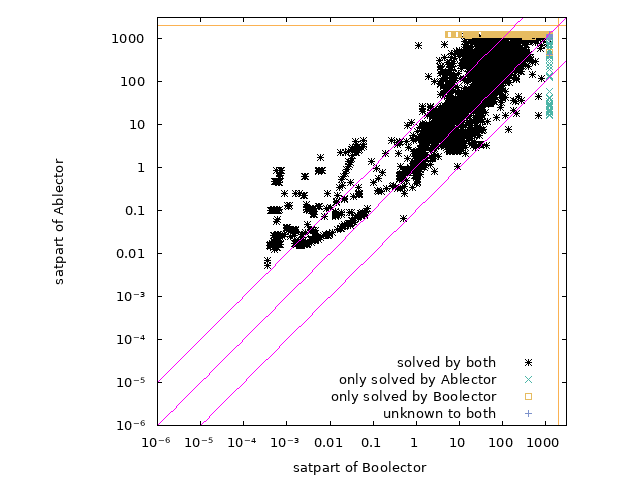
\includegraphics[width=0.7\textwidth]{plots/unsat/Boolector-vs-Ablector-satpart.png}
    \caption{\texttt{satpart} of Boolector vs \texttt{satpart} of Ablector in $\mu$s for unsatisfiable instances}
    \label{fig:evaluation:unsat:scatter}
\end{figure}

\begin{figure}[]
    \centering
        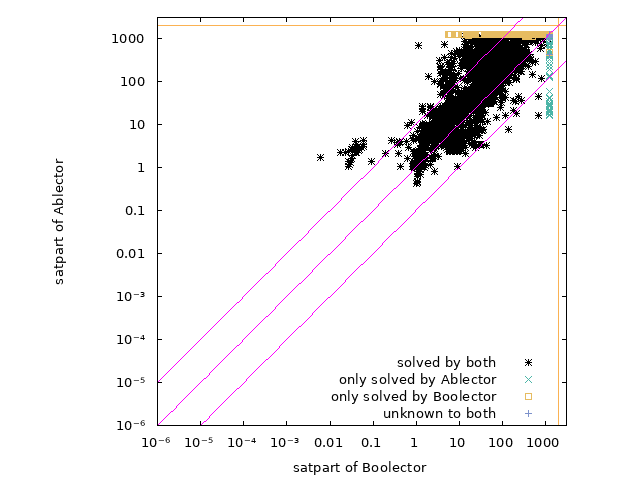
\includegraphics[width=0.7\textwidth]{plots/unsat/Boolector-vs-Ablector-satpart-big.png}
    \caption{\texttt{satpart} of Boolector vs \texttt{satpart} of Ablector in $\mu$s for unsatisfiable instances with satpart larger $1s$ in either dimension}
    \label{fig:evaluation:unsat:scatter-big}
\end{figure}
For any appearance of the \texttt{bvmul} and \texttt{bvsdiv} function within an instance we furthermore tracked the final abstraction level. Abstraction level 0 corresponds to the simple cases, level 1 corresponds to the msd based intervals, level 2 corresponds to the relations between functions and level 3 corresponds to the interval-wise full multiplication/division. If abstraction level 3 was reached, we further track the number of intervals added. This is of interest as it gives an estimate on the necessity of each refinement step: For example, if a refinement level would never appear as the final refinement step for an unsatisfiable instance, it is very unlikely that this abstraction is of much use. However looking at Figure \ref{fig:evaluation:unsat:level} we see that the final abstraction levels are somewhat distributed across the various abstraction steps and that all abstractions therefore help in solving certain instances.
Further, Figure \ref{fig:evaluation:unsat:interval} shows that for many instances full multiplication for a single interval (or very few intervals) are enough to produce the unsat result. This implies that the incremental, last refinement level also helps in solving certain instances.

\begin{figure}[ht]
    %\centering
    \begin{subfigure}[b]{0.5\textwidth}
        \centering
        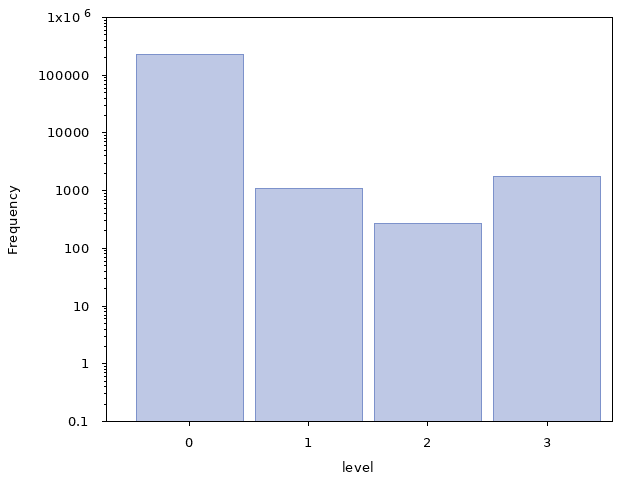
\includegraphics[width=\textwidth]{plots/unsat/level-MulNode.png}
        \caption{\texttt{bvmul}}
    \end{subfigure}
    \hfill
    \begin{subfigure}[b]{0.5\textwidth}
        \centering
        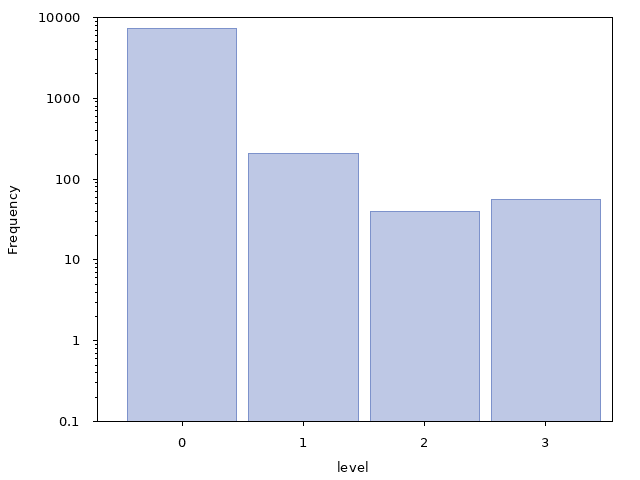
\includegraphics[width=\textwidth]{plots/unsat/level-SdivNode.png}
        \caption{\texttt{bvsdiv}}
    \end{subfigure}
    \caption{Final abstraction level of function applications: 0 are simple cases, 1 are bit shifts, 2 are UF relations and 3 is the interval-wise full multiplication/division step.}
    \label{fig:evaluation:unsat:level}
\end{figure}

\begin{figure}[ht]
    %\centering
    \begin{subfigure}[b]{0.5\textwidth}
        \centering
        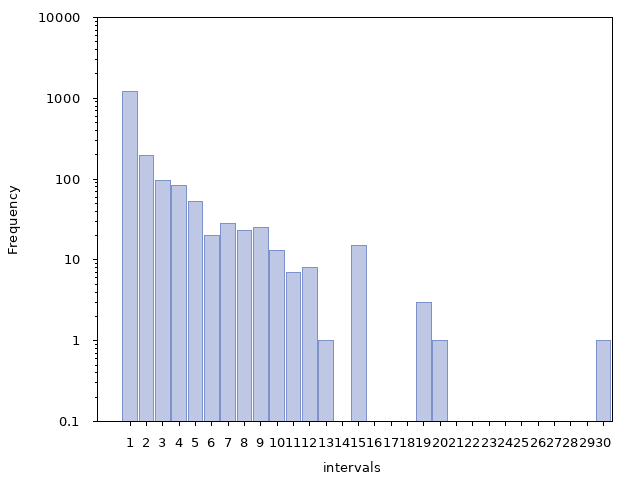
\includegraphics[width=\textwidth]{plots/unsat/bit-MulNode.png}
        \caption{\texttt{bvmul}}
    \end{subfigure}
    \hfill
    \begin{subfigure}[b]{0.5\textwidth}
        \centering
        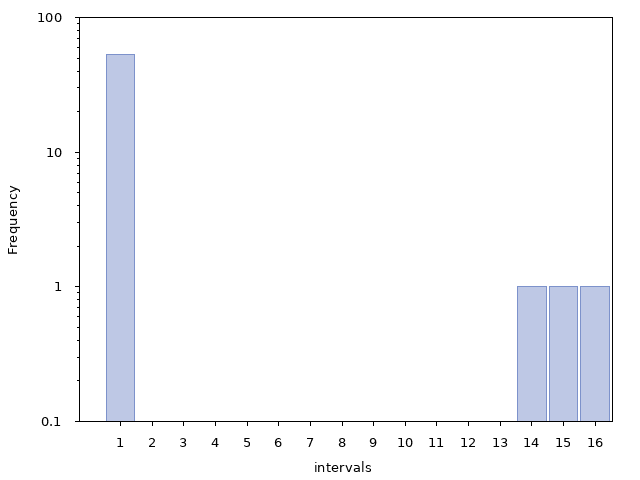
\includegraphics[width=\textwidth]{plots/unsat/bit-SdivNode.png}
        \caption{\texttt{bvsdiv}}
    \end{subfigure}
    \caption{Number of intervals added for multiplication/division in the final abstraction step.}
    \label{fig:evaluation:unsat:interval}
\end{figure}

%NOTE(steuber): Refinement time vs sat time?

\section{Satisfiable Instances}
For satisfiable instances on the other hand, Abletor's performance is worse than Boolector's: As we can see in Figure \ref{fig:evaluation:sat:scatter} and Table \ref{tab:evaluation:sat:solvedUnsolved}, Boolector is able to solve a lot of instances Ablector cannot currently solve and the running time Ablector takes for the solved instances cannot make up for this flaw.
It is also worth noting that, while about 500 timed out instances got stuck in the first refinement round, the rest of the timed out instances are evenly distributed across all refinement rounds.
\paragraph{}
While bounding the running time of each refinement round by an upper limit could avoid the problem of instances getting stuck in a certain step, we expect that the abstraction scheme's performance could further be improved in future work by integrating the abstractions directly into a solver like Boolector instead of building them as a layer on top. This would allow to make better use of the under-approximation techniques that are completely ignored for most abstraction steps in the current abstraction scheme.

\begin{figure}[]
    \centering
        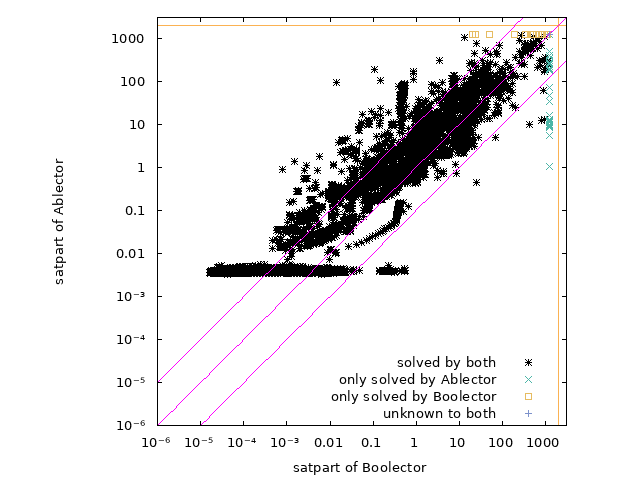
\includegraphics[width=0.7\textwidth]{plots/sat/Boolector-vs-Ablector-satpart.png}
    \caption{\texttt{satpart} of Boolector vs \texttt{satpart} of Ablector in $\mu$s for satisfiable instances}
    \label{fig:evaluation:sat:scatter}
\end{figure}

\begin{table}[ht]
    \begin{center}
    \begin{tabular}{cc|c|c|c}
        &&\multicolumn{2}{c|}{Boolector}&\\
        &&unsolved&solved&\\ \hline
        \multirow{2}{*}{Ablector}&unsolved& 579 & 474 & 1053 \\ \cline{2-5}
        & solved & 73 & 3400 & 3473 \\ \hline
        & & 652 & 3874 & 4526 \\
    \end{tabular}
    \end{center}
    \caption{Number of satisfiable instances solved by Boolector and Ablector}
    \label{tab:evaluation:sat:solvedUnsolved}
\end{table}